\subsubsection{ECP EZ: Fast, Effective, Parallel Error-bounded Exascale Lossy Compression for Scientific Data}

\paragraph{Overview}

Extreme scale simulations and experiments are generating more data than can be stored, communicated and analyzed. Current lossless compression methods suffer from low compression ratio and do not adequately address the limitations in storage bandwidth and storage space of projected Exascale systems. Existing lossy compressors, although enabling greater data reduction, are not covering the needs of many ECP applications.

The EZ project is extending and improving the SZ lossy compressor for structured and unstructured scientific datasets respecting user-set error controls. SZ offers an excellent compression ratio and compression time. Further work is essential, however, to improve our SZ lossy compressor for ECP scientific datasets, while ensuring that user-set error controls are respected. Specifically, we are maximizing the effectiveness of SZ's three core compression algorithms: prediction, quantization, and coding. The EZ project focuses on optimization of the compression quality, including improvement of compression ratio, memory cost minimization, parallelization, addition of more error controls, and integration of SZ into parallel I/O environments (PnetCDF, ADIOS, HDF5). Our goal is to produce a high-quality lossy compressor responding to the needs of ECP Exascale applications and experiment users. To this end, we are working with multiple ECP application teams, including ExaSky cosmology teams (HACC and Nyx), molecular dynamics simulations groups (EXAALT, QMCPACK), x-ray laser imaging experimentalists (ExaFEL), and computational chemists (NWChem-X) to optimize SZ for their applications and to harden SZ for production use.

\paragraph{Key Challenges}

There are several key challenges in the EZ project.
\begin{itemize}
\item One key challenge in designing an efficient compressor for HPC applications is the large
diversity of scientific simulation data, such as various dimensions, different scales, and dynamic data changes in both
space and time.
\item Another challenge is that the scientific data may have irregular characteristics. The simulation data may exhibit spiky changes in small local areas. For instance, all the key data in the HACC code are stored in six 1D arrays: three coordinate fields (xx, yy, zz) and three velocity fields (vx, vy, vz). It is hard to get a high compression ratio because of lack of correlations between adjacent particles in each array.
\item It is non-trivial to parallelize the lossy compressor SZ to get a high speed-up because of the relatively strong data dependencies in the data compression and decompression phase. The data prediction step, for example, relies on the neighboring data points for each data point, such that the entire compression/decompression has to be split into multiple blocks. How to perform the block-wise compression efficiently is an uneasy issue because block-wise prediction may degrade the prediction accuracy.
\item Integrating SZ into parallel I/O libraries (such as PnetCDF and HDF5) is non-trivial, because these I/O libraries are designed and implemented differently with various interfaces. We need to develop the integration codes based on the I/O libraries' interface with minimal cost.
\end{itemize}

\paragraph{Solution Strategy}

As for the first challenge, we keep a close communication with ECP application users to understand their specific demands on the lossy compression. For instance, we have a weekly meeting with ExaSky team to discuss the required error bounds and compression quality of cosmology simulation data. We also provide multiple types of error bounds (such as absolute error bound, PSNR, relative error bound) allowing users to control the errors in different ways.

As for the second challenge, we develop some particular compression techniques based on specific data features across different applications.

As for the third challenge, we split the entire dataset into multiple blocks based on the number of threads/ranks and conduct an adaptive prediction method to optimize the prediction accuracy dynamically.

We overcome the last challenge by understanding the principle of the I/O libraries (either reading the related documents or communicating with the I/O library developers closely).

\paragraph{Recent Progress}

SZ has been released as an open source on GitHub (http://github.com/disheng222/SZ). Figure \ref{fig:sz-principle} (a) demonstrates the core step (data prediction and linear-scaling quantization) in SZ lossy compression using a 2D dataset. Our customized improved compression techniques for different datasets mainly focus on various prediction methods based on data features. 
Figure \ref{fig:sz-principle} (b) demonstrates the visual quality of decompressed data for ExaSky-NYX VX field. We can see that SZ has a pretty high visual quality even with a high compression ratio up to 156:1. 

\begin{figure}[htb]
\centering
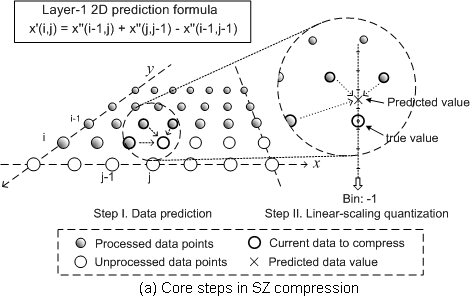
\includegraphics[width=2.8in]{projects/2.3.4-DataViz/2.3.4.06-EZ/sz-illu.png}
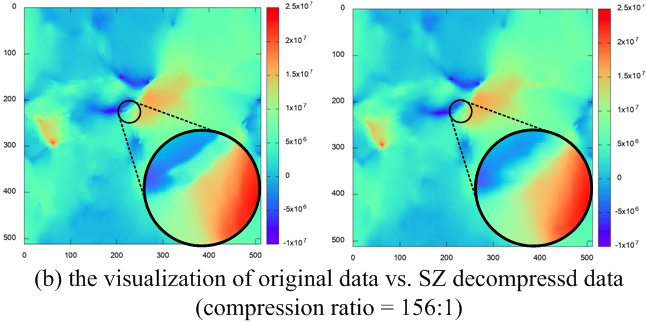
\includegraphics[width=3.2in]{projects/2.3.4-DataViz/2.3.4.06-EZ/Visual-quality-NYX-SZ.png}
	\caption{\label{fig:sz-principle}Illustration of data prediction in SZ and visual quality of decompressed data for ExaSky-NYX VX field}
\end{figure}

We have improved the compression quality for some ECP applications significantly. For instance, we develop PaSTRI code that can significantly improve the compression ratio for GAMESS two-electron integral datasets by leveraging the potential scaled repeated patterns. We also implemented effective compression method supporting point-wise relative error bounds for the ExaSky project and studied its lossy compression quality with multiple resolutions. Experiments with point-wise relative error bound based compression shows that our solution leads to 31\%-210\% higher compression ratio than other lossy compressors do.

We developed the multi-thread OpenMP version for SZ and evaluate the parallel compression performance, as presented in Figure \ref{fig:openmpperformance} (a). It is observed that the compression can obtain a speed-up of 250+ and the overall performance using lossy compression+I/O can be improved 15X compared with the data I/O without lossy compressor.
we can observe that the OpenMP version of SZ obtains about 6:1$\sim$16:1 performance gain when using 8$\sim$64 threads to do the compression/decompression in parallel. Decompression has higher performance gain than compression as the number of cores grow because it does not need to construct the Huffman tree.

We completed the integration of SZ into three popular I/O libraries (PnetCDF, ADIOS, and HDF5). Figure \ref{fig:openmpperformance} (b) and (c) present the performance evaluation using PnetCDF integrated with SZ.

\begin{figure}[htb]
\centering
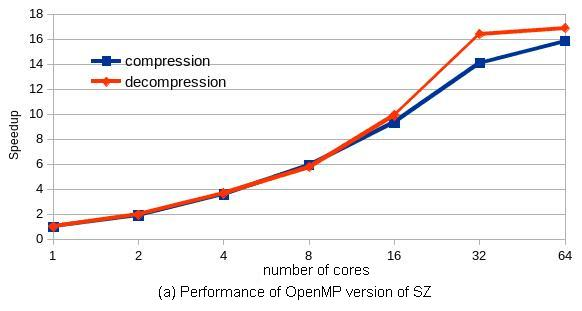
\includegraphics[width=2.8in]{projects/2.3.4-DataViz/2.3.4.06-EZ/openmp-perf-SZ.jpg}
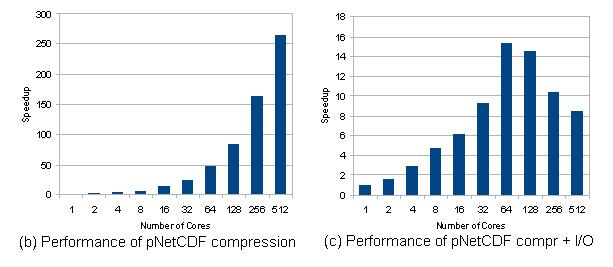
\includegraphics[width=3.5in]{projects/2.3.4-DataViz/2.3.4.06-EZ/pNetCDF-perf-SZ.jpg}
\caption{Performance evaluation of SZ with OpenMP and PnetCDF}
\label{fig:openmpperformance}
\end{figure}


\paragraph{Next Steps} Our next efforts are: 

\textbf{Improve compression ratio by leveraging the smoothness of the data in the time dimension.} (1) Explore techniques for compression in time dimension; (2) Integration of compression in time dimension. (3) Test and performance evaluation on available CORAL systems

%\textbf{Support advanced error controls allowing the user to specify relative error bounds and to control the error distribution.} We will write a report describing the integration of additional error controls (relative error bound and control of error distribution) in SZ.
